%中間審査概要テンプレート ver. 3.0

\documentclass[uplatex,twocolumn,dvipdfmx]{jsarticle}
\usepackage[top=22mm,bottom=22mm,left=22mm,right=22mm]{geometry}
\setlength{\columnsep}{10mm}
\usepackage[T1]{fontenc}
\usepackage{txfonts}
\usepackage[expert,deluxe]{otf}
\usepackage[dvipdfmx,hiresbb]{graphicx}
\usepackage[dvipdfmx]{hyperref}
\usepackage{pxjahyper}
\usepackage{secdot}





%タイトルと学生番号,名前だけ編集すること
\title{\vspace{-5mm}\fontsize{14pt}{0pt}\selectfont クラウドファンディングの成功要因分析}
\author{\normalsize プロジェクトマネジメントコース 矢吹研究室 1342066 島田樹}
\date{}
\pagestyle{empty}
\begin{document}
\fontsize{10.5pt}{\baselineskip}\selectfont
\maketitle





%以下が本文
\section{背景}
クラウドファンディング\cite{wiki}とは,自らのアイディアやプロジェクトをネット上でプレゼンテーションすることで,支援者を集めて資金を獲得する手法である.SNSの発達に伴いプロジェクトの数も増加し,市場も年々増加している\cite{visualizing}.幅広い分野と規模での応募が可能で,ベンチャー企業のプロジェクトや学生の研究費用の獲得などが多かったが,大手企業も支援者数から売れることを確実視されたプロダクトを販売者できるとして,マーケティングの一環として活用されるようになってきた.

課題研究において,調達資金の時間変化を調査しグラフ化したところ,資金が集まり始める時期には実行者が何らかの行動をしていると考えた.資金が集まる直前の実行者の行動を分析すればクラウドファンディングにおけるプロジェクトの成功率を上げることができるのではないかと考えられる.


\section{目的}
日本での大手クラウドファンディングサイトであるREADYFORとMakuakeで掲載されているプロジェクトから,調達資金の変化を可視化する.その結果をもとに,動画の投稿やSNSでの告知などの多くの資金を集める直前にするべきプロジェクト実行者の行動の参考となる指標を作ることを目的とする.


\section{手法}
クラウドファンディングサイトを,毎日定時に監視し,データ収集を行う.プロジェクトの調達資金の変化をグラフ化しパターン分けをする,成功しているプロジェクトが資金を獲得している時にしている行動を考察する.


\section{想定される成果物}
プロジェクトの資金調達の情報からグラフ化しパターン分けをする.調達された日に行われた行動が成功要因であるかを判別する.課題研究においてグラフのパターンは以下の4種類に分類された.
\begin{enumerate}
 \item 目標金額以上集まった後,それ以降金額が伸びなかったプロジェクト
 \item 目標金額に対して金額があまり伸びず,終了直前になって急激に伸びて目標金額に達したプロジェクト 
 \item 最初に金額が少し伸びた後,ほとんど金額が伸びず失敗したプロジェクト
 \item 目標金額に対して金額が伸びていたが達するまでに至らず,終了直前に急激伸びるが失敗したプロジェクト
\end{enumerate}
このグラフから,金額が大きく伸び始めた頃に実行者がしていた行動を分析し,成功要因を出す.
\begin{figure}[h]
\centering
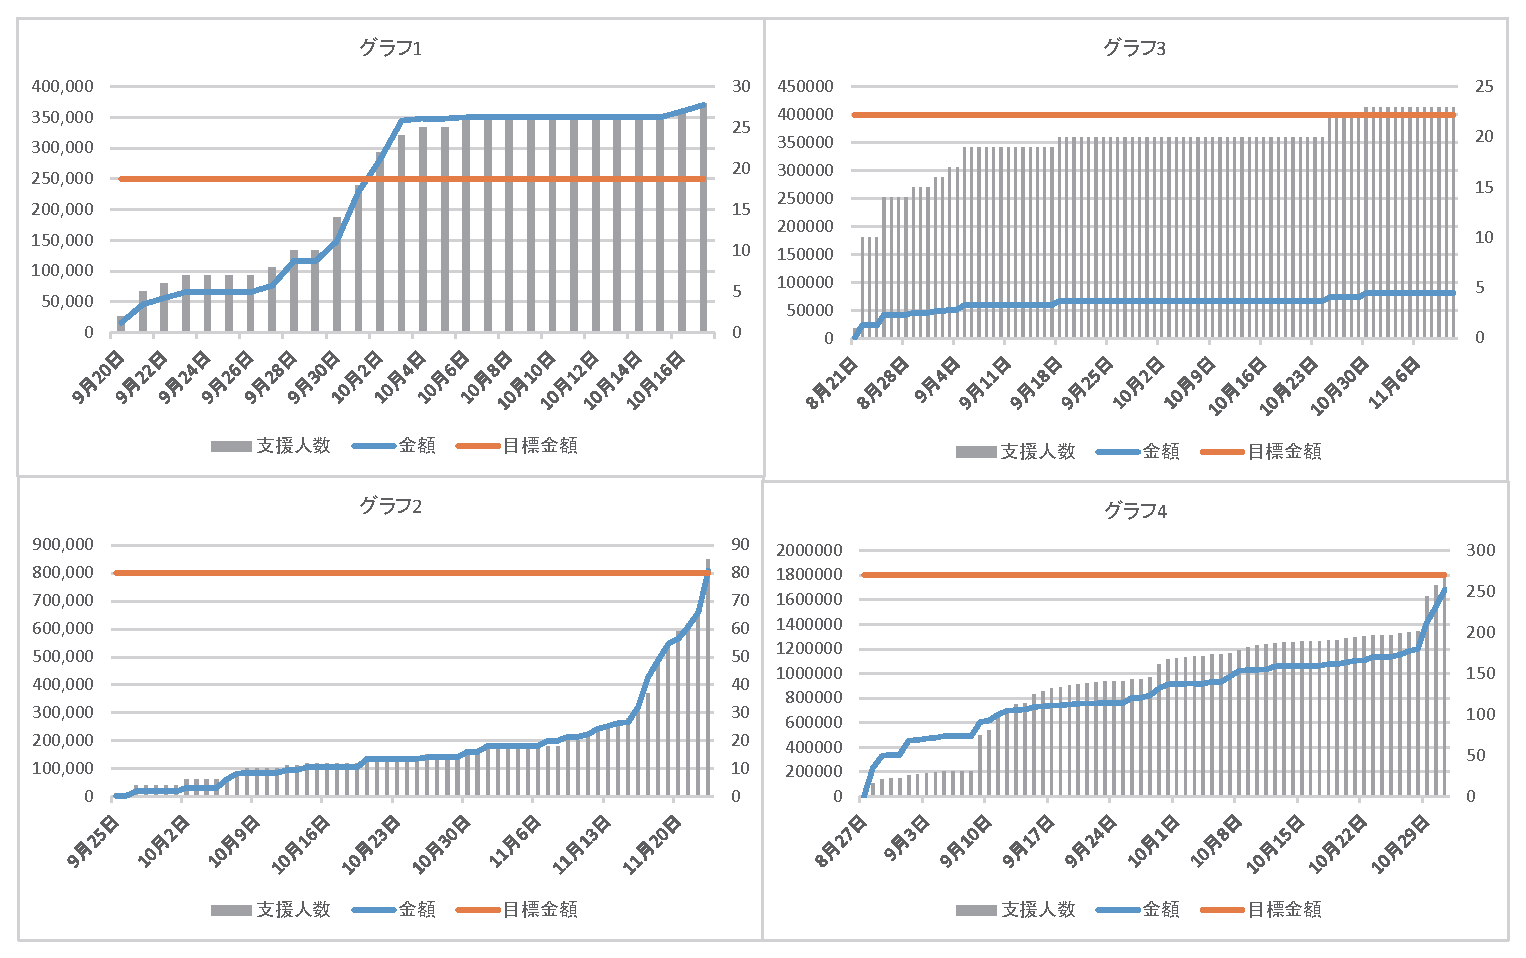
\includegraphics[width=8cm,clip]{images.pdf}
\caption{調達資金の時間変化4種類}\label{サンプル図}
\end{figure}
\section{進捗状況}
現在までに約5か月分のデータを集め,継続して収集している.集めたデータから欲しい情報だけを自動的に抜き取る方法を模索している.
\section{今後の計画}
今後は,引き続きデータを集めて資金調達の成功要因であるものの的中率を上げる.


\bibliographystyle{junsrt}
\bibliography{biblio}%「biblio.bib」というファイルが必要.

\end{document}
